\documentclass{beamer}
\usetheme{Warsaw}
% \usetheme{Goettingen} alternative themes
% \usetheme{Hannover}
% \usetheme{Marburg}
% \usetheme{PaloAlto}
\usepackage[utf8]{inputenc}
\usepackage{polski}
\usepackage[polish]{babel}
\usepackage{graphicx}
\usepackage{mathtools}

\title{Digital timestamps}
\author{Kangaroos Team}
\institute{APPSEC}
\date{06.04.2014}
\begin{document}

\begin{frame}
\titlepage
\end{frame}

\begin{frame}
	\frametitle{Po co?}
	\begin{block}{Time Stamp Authority}
   The TSA is a TTP (Trusted Third Party) that creates time-stamp tokens in order to indicate that a datum existed at a particular point in time
   \end{block}
	
	\begin{block}{Możliwe zastosowania}
		\begin{itemize}
			\item verify that a digital signature was
   applied to a message before the corresponding certificate was revoked
   thus allowing a revoked public key certificate to be used for
   verifying signatures created prior to the time of revocation
			\item indicate the time of submission when a deadline is
   critical
   			\item indicate the time of transaction for entries in a
   log
		\end{itemize}
	\end{block}
\end{frame}

\begin{frame}
	\frametitle{Wybrane wymagania co do TSA}
		\begin{enumerate}
			\item to use a trustworthy source of time.
			\item to include a trustworthy time value for each time-stamp token.
			\item to include within each time-stamp token an identifier to
         uniquely indicate the security policy under which the token was
         created.

   			\item to only time-stamp a hash representation of the datu
   			\item not to examine the imprint being time-stamped in any way (other than to check its length, as specified in the previous bullet).

   			\item not to include any identification of the requesting entity in the time-stamp tokens.

   			\item to sign each time-stamp token using a key generated exclusively for this purpose and have this property of the key indicated on  the corresponding certificate.
		\end{enumerate}
\end{frame}

\begin{frame}
	\frametitle{O kluczu prywatnym}  
	The certificate corresponding to the private key MUST contain only one instance of the extended key usage field extension as defined in [RFC2459] Section 4.2.1.13 with KeyPurposeID having value: \textbf{id-kp-timeStamping}.  This extension MUST be critical.
\end{frame}


\begin{frame}
	\frametitle{Bezpieczeństwo}
	  When a TSA shall not be used anymore, but the TSA private key has
      not been compromised, the authority's certificate SHALL be
      revoked.  
      
      reasonCode (CRL extensions):
      \begin{itemize}
      \item unspecified (0)
      \item affiliationChanged (3)
      \item superseded (4) 
      \item cessationOfOperation (5)
      \end{itemize}  In that case, at any
      future time, the tokens signed with the corresponding key will be
      considered as invalid, but tokens generated before the revocation
      time will remain valid.  
      
      When the reasonCode extension relative to
      the revoked certificate from the TSA is not present in the CRL
      entry extensions, then all the tokens that have been signed with
      the corresponding key SHALL be considered as invalid.
\end{frame}

\begin{frame}
	\frametitle{Bezpieczeństwo}
	  When the TSA private key has been compromised, then the
      corresponding certificate SHALL be revoked.  
      \begin{itemize}
	\item      reasonCode: keyCompromise (1) or extension not present
      \end{itemize}
      
      Any token signed by the TSA using that private key cannot be trusted
      anymore. In case the private key does become compromised, an audit trail of all tokens generated by the TSA MAY provide a means to discriminate between genuine and false backdated tokens.  Two time-stamp tokens from two different TSAs is another way to address this issue.
\end{frame}


\begin{frame}
	\frametitle{Bezpieczeństwo}
	  The TSA signing key MUST be of a sufficient length to allow for a
      sufficiently long lifetime.  Even if this is done, the key will
      have a finite lifetime.  
      
      sThus, any token signed by the TSA SHOULD
      be time-stamped again (if authentic copies of old CRLs are
      available) or notarized (if they aren't) at a later date to renew
      the trust that exists in the TSA's signature. time-stamp tokens
      could also be kept with an Evidence Recording Authority to
      maintain this trust.
\end{frame}

\begin{frame}
	\frametitle{Zdobywanie timestampa} 
	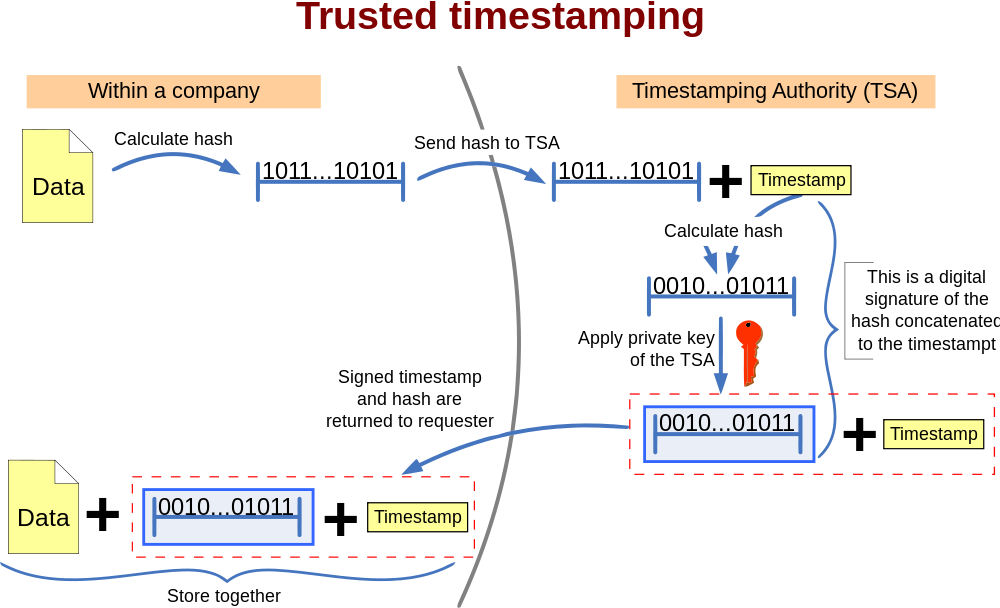
\includegraphics[width=300px]{Trusted_timestamping.png}
\end{frame}

\begin{frame}
	\frametitle{Weryfikacja timestampa} 
	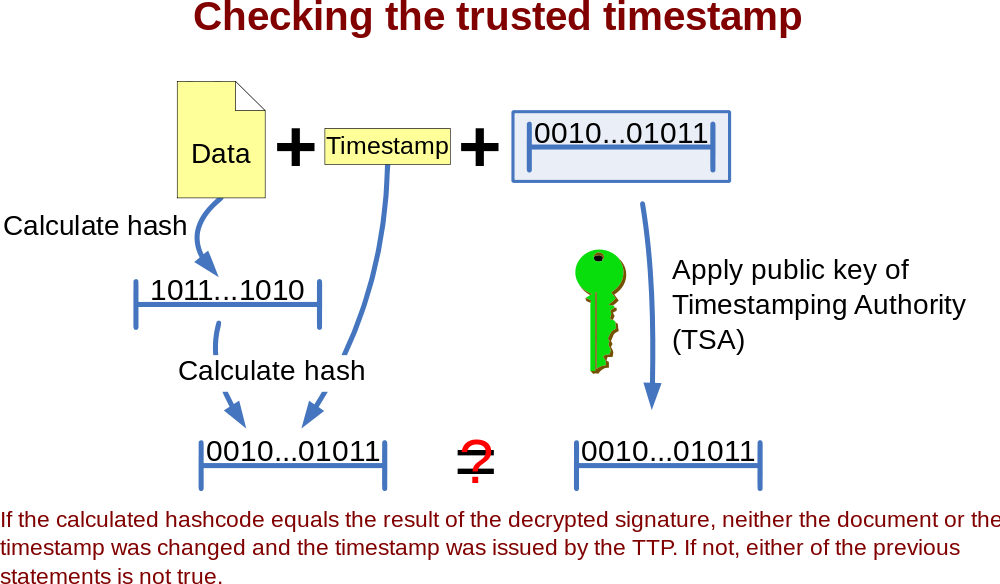
\includegraphics[width=300px]{Checking_timestamp.png}
\end{frame}  

\end{document} 